\documentclass[tikz]{standalone}
\usetikzlibrary{calc}

  \usepackage[no-math]{fontspec}
  \setmainfont{TeXGyreTermes-Regular}[
       BoldFont       = TeXGyreTermes-Bold ,
       ItalicFont     = TeXGyreTermes-Italic ,
       BoldItalicFont = TeXGyreTermes-BoldItalic,
       NFSSFamily     = ntxtlf]
  \setsansfont{TeX Gyre Heros Regular}[
       Scale=.9,
       BoldFont       = TeX Gyre Heros Bold,
       ItalicFont     = TeX Gyre Heros Italic,
       BoldItalicFont = TeX Gyre Heros BoldItalic]
  \setmonofont[StylisticSet={1,3},Scale=.9]{inconsolata}
  \usepackage{newtxmath}
\begin{document}

\definecolor{Maroon}{cmyk}{0, 0.87, 0.68, 0.32}

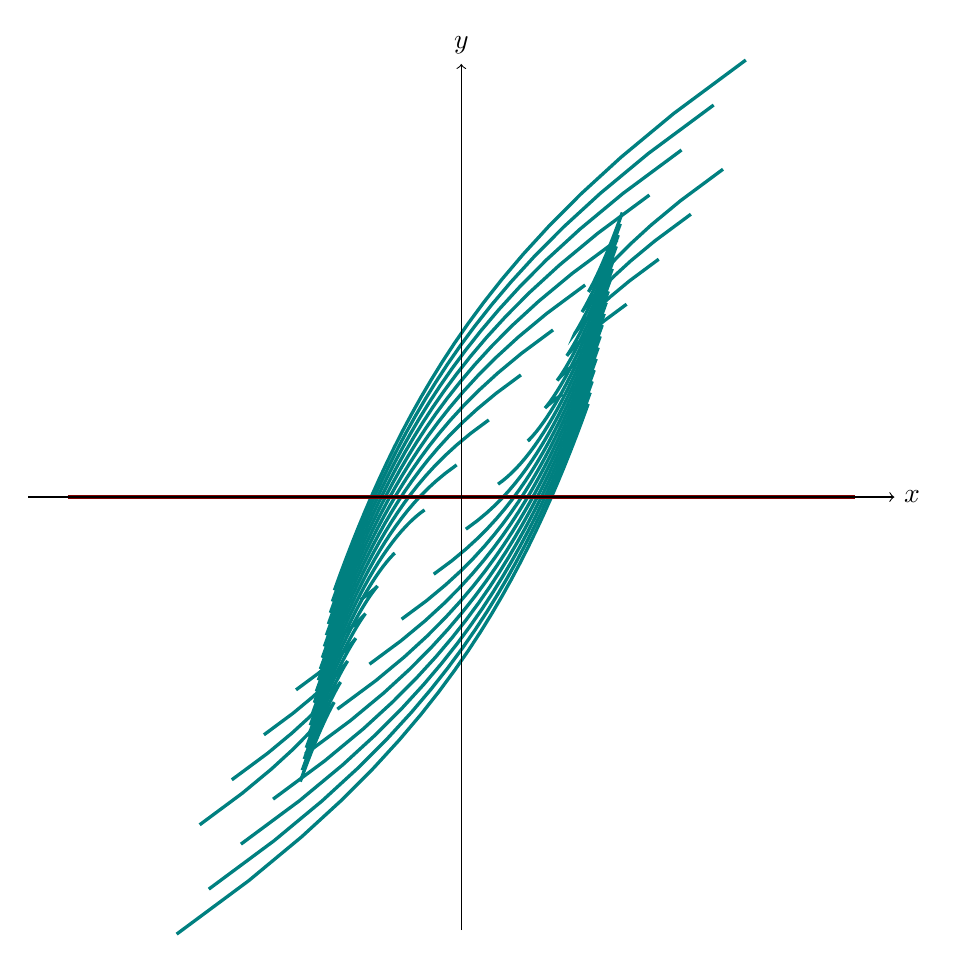
\begin{tikzpicture}
\def\xmax{5} \def\xmin{-5}
\def\ymax{5} \def\ymin{-5}


\foreach \C in {-2,-1.8,...,1.5}
\draw[very thick, color=teal] plot[domain=0.7:2.8] ({(2/3)*\x + \C/(\x^2)},{(1/3)*\x^2 + (2*\C)/\x});
\foreach \C in {-2,-1.8,...,1.5}
\draw[very thick,color=teal] plot[domain=-2.8:-0.7] ({(2/3)*\x + \C/(\x^2)},{(1/3)*\x^2 + (2*\C)/\x});
\draw[ultra thick, Maroon] (-5,0)--(5,0);
\draw[->] (\xmin-.5,0)--(\xmax+.5,0) node[right] {$x$};
\draw[->] (0,\ymin-.5)--(0,\ymax+.5) node[above] {$y$};
\end{tikzpicture}
\end{document}